\section{About Blockchain}

To begin with, this chapter will give an overview of the general purpose, the contained components and the fundamental functionality of a blockchain. 

\subsection{General Purpose}
In general, a blockchain can be described as a digital data structure that can be understand as a shared and distributed database, containing a continuous expanding and chronological log of transactions \shortcite{andoni2019blockchain}. Besides, various types like digital transactions, data records and executables can be stored in this digital data structure. The data transmission in a blockchain is comparable with copying data from one computer to another. However, the resulting challenge is that the system needs to ensure that the data is copied just once \shortcite{andoni2019blockchain}. For example, in the domain of cryptocurrencies, this is equal to sending a coin from one wallet to another. In this case, the system needs to validate that this coin is spended just once and there is no double-spending. A conventional solution for this problem is a third intermediary. To come back to the stated example, the third intermediary is represented by a traditional bank, which store, protect and continuously update the valid state of the ledger \shortcite{andoni2019blockchain}. But, in some cases central management is not practicable or reasonable. Reasons for this are possible intermediary costs or a high degree of trust of the users into the intermediary who operates the system. Further, central management has a significant disadvantage because of a single point of failure. Hence, the centralized system is fragile to technical problems as well to external malicious attacks \shortcite{andoni2019blockchain}.
Consequently, the main reason of bockchain technologies is the removal of such third trusted intermediaries through a distributed network of various users, who cooperating together to verify transactions and protect the validity of the ledger

\subsection{Architecture}
This subsection covers the architectural design of a blockchain and presents the contained components in detail. Due to the plurality of the blockchain technologies, each of the technology slightly differs in design and components. The following explanations are oriented torwards the Ethereum blockchain implementation, which is also used as the underlying ICT to implement the open simulation platform.

\subsubsection{World State}
\label{sec:world_state}
Referring to the \textit{Yellow Paper} \shortcite{wood2014ethereum}, Ethereum can be seen as a transaction-based state machine. What does that mean? At the beginning, Ethereums state machine starting with a so called \textit{"genesis state"}. This is analogous to a blank sheet. On this state, no transactions have happened on the network. Next, transactions are executed and the state of the Ethereum world changes into a new state. Further, transactions are executed incrementally and morph it into some final state. Consequently, the final state is accepted as the canonical version of the world of Ethereum and represents at any times the current state.

\begin{figure}[htbp]
	\centering
	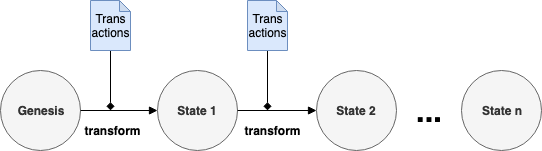
\includegraphics[width=.9\linewidth]{./figures/state_transition.png}
	\caption{World State: Transition of States}
	\label{figure:state_transition}
\end{figure}

In more detail, the world state arises out of a mapping of a key value pair for every account which exists on the Ethereum network \shortcite{wood2014ethereum}. The key constitutes the address of an Ethereum account and the value presents the account's state, which contains detailed information of this account. 
However, the world state is not stored on the blockchain itself. This mapping is stored and maintained in a modified data structure called a \textit{Merkle Patricia tree}. This tree is stored off-chain in a simple database backend (i.e. on a computer running an Ethereum client), also known as the \textit{state database} in the Ethereum world \shortcite{wood2014ethereum}. To get a better understanding of the operating principles of the blockchain, it is necessary to get an idea of how a \textit{Merkle Patricia tree} works. A \textit{Merkle Patricia tree} is a type of binary tree, which consists of a set of nodes. It has a large amount of 
\textit{leaf nodes}, containing the underlying data. Further, a set of intermediate nodes, where each node is the hash of its two children, and finally, one single root node, representing the top of the tree which is also build out of its two child nodes \shortcite{buterin2013next} \shortcite{wood2014ethereum}.
As mentioned before, the \textit{leaf nodes} contain the stored data by splitting these data into chunks. Afterwards, these chunks are splitted into buckets. Then, each bucket gets hashed and the same process repeats, traversing upwards the tree, until the total number of hashes remaining becomes only one and the root node is reached \shortcite{ethereum_blog}. 

\begin{figure}[htbp]
	\centering
	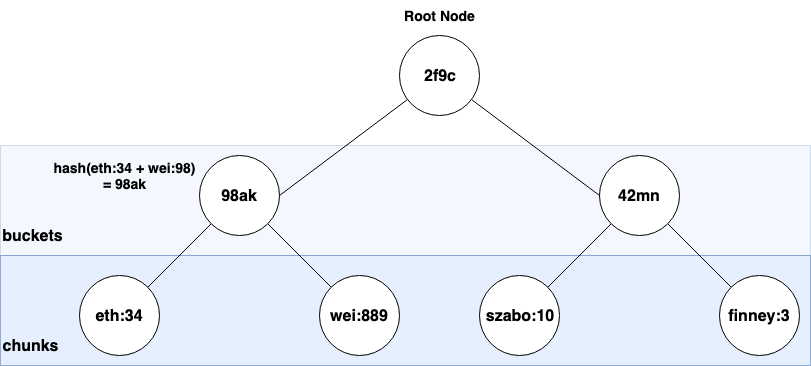
\includegraphics[width=.9\linewidth]{./figures/merkle_tree.png}
	\caption{Example of a Patricia Merkle tree}
	\label{figure:merkle_tree}
\end{figure}

Therefore, any change to the underlying data, stored in a \textit{leaf node}, causes a change of the hash of the node. Each parent's node hash depend on the data of its children. Due to this, any change to the data of a child node causes the parent hash to change. This procedure repeats traversing upwards until the root node. Hence, any change to the data at the leaf nodes effects the root hash \shortcite{ethereum_wiki}. 

\begin{figure}[htbp]
	\centering
	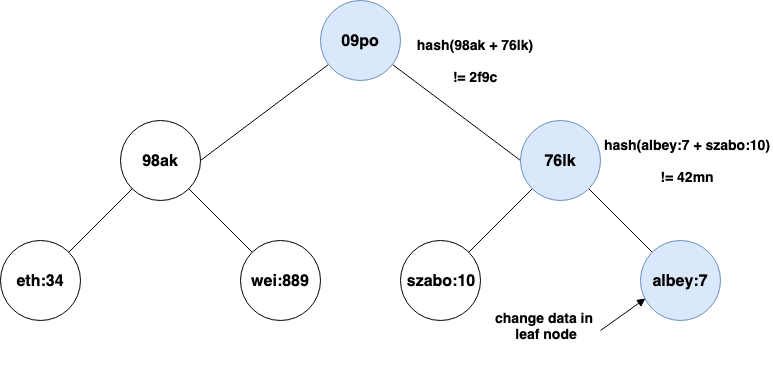
\includegraphics[width=.9\linewidth]{./figures/merkle_tree_change.png}
	\caption{Example of a data change in a leaf node}
	\label{figure:merkle_tree_change}
\end{figure}

Because of this characteristic, it is not necessary to compare the data of the entire tree. It is sufficient to compare the single root hash to ensure that all the data are the same. This property is very important, because it makes it possible to store only the hash of the root node to represent a state of the ethereum world. 

\subsubsection{Block} 
\label{sec:block}
As described in section \ref{sec:world_state}, whenever transactions are executed, the state of the Ethereum world changes into a new state. Every state and the belonging transactions, which transform the prior state into the new state, is cumulated in a so called block. That means, states are represented by blocks. As you can see in figure \ref{figure:state_transition}, the history of the Ethereum world is a linkage of states, or in other words, blocks. That is where the name blockchain comes from. A blockchain is a sequence of blocks, which holds a complete list of transaction records \shortcite{zheng2017overview}. 
Moreover, a block is a collection of different relevant informations and consists of the \textit{block header} and the \textit{block body}, which contains the list of transactions. Following \textit{Ethereums Yellow Paper} \shortcite{wood2014ethereum}, the subsequent pieces of information are contained in the \textit{block header}:

\begin{description}
	\item[Parent Hash:] This is the hash of the parents block's header. Therefore, every block points to his ancestor. Due to this contained attribute, a chain arises out of the single blocks.
	\item[Beneficiary:] The miners address to which all block rewards from the successful mining of a block are transferred.
	\item[State Root:] This is the hash of the root node of the state tree, after a block and its transactions are finalized. As mentioned in section 
	\ref{sec:world_state}, the state tree is the one and only global state in the Ethereum world. It is used as a secure unqiue identifier for the state and the state root node is cryptographically dependent on all internal state tree data.
	\item[Transactions Root:] This is the hash of the root node of the transaction tree. This tree contains all transactions in the block body. In contrast to the state tree, there is a separate transactions tree for every block. 
	\item[Receipts Root:] Every time a transaction is executed, Ethereum generates a transaction receipt that contains information about the transaction execution. This field is the hash of the root node of the transactions receipt tree and like the transaction tree, there is a seperate receipt tree for every block.
	\item[Difficulty:] This is a measure of how hard it was to mine this block – a quantity calculated from the previous block’s difficulty and its timestamp
	\item[Number:] This is a quantity equal to the number of blocks that precede the current block in the blockchain.
	\item[Gas Limit:] This is a quantity equal to the current maximum gas expenditure per block. Each transaction consumes gas. The gas limit specifies the maximum gas that can be used by the transactions included in the block. It is a way to limit the number of transactions in a block.
	\item[Gas Used:] This is a quantity equal to the total gas used in transactions in this block.
	\item[Timestamp:] This is a record of Unix’s time at this block’s inception.
	\item[Nonce:] This is an 8-byte hash that verifies a sufficient amount of computation has been done on this block. Further, it is a number added to a hashed block that, when rehashed, meets the difficulty level restrictions. The nonce is the number that blockchain miners are solving for.
\end{description}

So far, we introduced Ethereum as a transaction-based state machine, transforming one state into another through the execution of transactions. Further, we explained how these individual states are stored and emphasises the meaning of these storage. Moreover, we pointed out that an Ethereum state is represented by blocks and described all relevant informations contained in it.
However, we didn't introduce how many transactions be part of a block and who build and validate a block? To answer this, we introduce the transaction object and his life cycle in depth.


\subsubsection{Transaction}
\label{sec:transaction}
To start with, a transaction is the basic method for Ethereum accounts to interact with each other. Further, in the Ethereum world exists two different types of transactions. Those, which result in a so called \textit{message call}, which can be seen as a traditional transaction, and those which result in a \textit{contract creation} \shortcite{wood2014ethereum}. 
Though, both different types of transaction share the following common attributes \shortcite{wood2014ethereum}:

\begin{description}
	\item[Nonce: ] This attribute is discontiguous of the block attribute. In contrast to the block attribute, the nonce of a transaction keep track of the total number of transactions that an account has executed. 
	\item[Gas Price: ] As mentioned in section \ref{sec:block}, each transaction consume gas. Gas can be seen as fees. This attribute presents the price per unit of gas for a transaction \footnote{A website to see current gas prices: https://ethgasstation.info/index.php}. 
	\item[Gas Limit: ] This attribute is similiar to the block attribute of the same name. In this case, it is a quantity equal to the current maximum gas expenditure per transaction.  
	\item[To: ] In case of a \textit{message call}, this attribute contains the address of the recipient. Otherwise, in case of a \textit{contract creation} this value remains empty. 
	\item[Value: ] In case of a \textit{message call}, this attribute contains the amount of Wei, which will be transferred to the recipient. In the case of a \textit{contract creation}, this value contains the amount of Wei as a intial endowment of the contract.
\end{description}

\subsubsection{Transaction Life Cycle}
\label{sec:transaction_lifecycle}
Next, the life cycle of a transaction will be outlined. We will take a simple \textit{message call} as an example and will pass through the entire flow of how this transaction gets executed and permanently stored on the blockchain. During this process, many basic concepts of a blockchain will be introduced. 

To begin with, someone want to send an abitrary amount of ether to someone else. Consequently, a transaction with the respective attributes, which are stated in section \ref{sec:transaction}, will be created. As a first step, this transaction will be signed. That means, the one who wants to execute the transaction needs to proof the ownership of the account. Otherwise, someone else could execute a transaction on your behalf. The way to proof this is by signing the transaction with the corresponding private key of this account \shortcite{transaction_life_cycle}. 
Next, the signed transaction is submitted to the related Ethereum node. Then, the node will validate the signed transaction. After a successful validation, the node will send the transaction to it's peer nodes, who again send it to their peer nodes and so on \shortcite{transaction_life_cycle}. As soon as the transaction is broadcast to the network, the related node will declare a transaction id, which is the hash of the signed transaction and can be used to track the status of the transaction \footnote{A Website to track transactions: https://etherscan.io/}. Further, figure \ref{figure:node_network} describes a Ethereum network. As you can see, it contains a mix of miner nodes and non miner nodes. The non miner nodes can be distinguished into different types of nodes with different behavior, which are explained in detail in section \ref{sec:nodes}. The miner nodes are the ones who processing transactions into blocks \shortcite{transaction_life_cycle}. 

\begin{figure}[htbp]
	\centering
	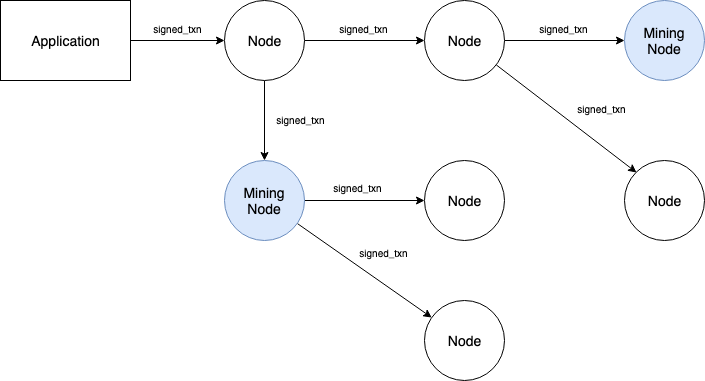
\includegraphics[width=.9\linewidth]{./figures/node_network.png}
	\caption{Node network demonstrating a transaction broadcast}
	\label{figure:node_network}
\end{figure}

Mining nodes contain and maintain a pool of transactions where they collect incoming transactions. They sort the transactions by gas price. However, there are no specific rules how the nodes sort the transactions. A common configuration is to sort the transaction by gas price in a descending order to optimize for a higher pay \shortcite{transaction_life_cycle}.

\begin{longtable}{c|c}
	\hline
	\hline
	Signed Transaction & Gas Price \\
	\hline
	hashOfTransaction1 & 15 Gwei \\
	hashOfTransaction2 & 13 Gwei \\
	hashOfTransaction3 & 11 Gwei \\
	hashOfTransaction4 & 10 Gwei \\
	hashOfTransaction5 & 7 Gwei \\
	\hline
	\hline
	\caption{Transaction Pool of Mining Node}
	\label{table:sorted_gas_prices}
\end{longtable} 

Further, the mining node takes transactions from the pool and processes them into a pending block. Moreover, a block can only contain a certain number of transactions due to the block attribute \textit{gas limit}, mentioned in section \ref{sec:block}. That means, the mining node can only process so many transactions into one block until the gas limit is reached \footnote{A website to see current attributes: https://ethstats.net/}. For example, imagine that the current \textit{gas limit} of a block is 28 Gwei. Next, we look at the transaction pool of a mining node in table \ref{table:sorted_gas_prices}. As you can see, two blocks are required to process all transactions from the pool. The first two transactions are contained in the first block. Furhtermore, the second block contains the remaining three transactions. 
So far, it is described how a pending block will be created and the transaction limit of a block is explained. In the next section \ref{sec:mining}, the process of a pending block to a valid block is outlined in depth. Finally, after the validation process of a block is finished successfully, the life cycle of a transaction is over. That means, the transaction is anchored in the blockchain and modified the world state as mentioned in section \ref{sec:world_state}.

\subsubsection{Mining}
\label{sec:mining}
Next, the validation of a block will be outlined. In general, each mining node in the network can generate or propose a block. The emerging question is, how will the newly generated block accepted by the remaining network members? This process is called \textit{consensus mechanism} \shortcite{andoni2019blockchain}. 

\subsubsection{Nodes}
\label{sec:nodes}


\clearpage

